%%% The main file. It contains definitions of basic parameters and includes all other parts.


%% Settings for two-sided (duplex) printing
\documentclass[10pt,a4paper]{article}
\let\openright=\cleardoublepage

%% Character encoding: usually latin2, cp1250 or utf8:
\usepackage[utf8]{inputenc}

%% It's 2019
\usepackage[default]{droidserif}
\usepackage[T1]{fontenc}

%% Further useful packages (included in most LaTeX distributions)
\usepackage{amsmath}        % extensions for typesetting of math
\usepackage{amsfonts}       % math fonts
\usepackage{graphicx}       % embedding of pictures
\usepackage{tikz}
%\usetikzlibrary{shapes,fit,positioning,snakes,mindmap,trees,decorations.text,arrows.meta}
%\makenomenclature
\usepackage{algorithm,algpseudocode}
\usepackage{booktabs}
\usepackage{mwe}
\usepackage{afterpage}
\usepackage{pgfgantt}
\usepackage{pdflscape}
\usepackage{geometry}
\usepackage{enumitem}
\usepackage{float}
\usepackage{framed}
\usepackage{titlesec}
\usepackage{listings}
\usepackage{xcolor}
\usepackage{longtable}
\usepackage{makecell}
\usepackage[toc,page]{appendix}
\usepackage{multirow}
\usepackage{tocbibind}
\usepackage{etoolbox}
\usepackage{fancyvrb}
\usepackage{animate}
\usepackage{caption}
\usepackage{subcaption}

\lstset{basicstyle=\ttfamily,
	showstringspaces=false,
	commentstyle=\color{red},
	keywordstyle=\color{blue}
}

\usepackage{pdfpages}

\usepackage[textsize=tiny,backgroundcolor=yellow!50, linecolor=black!25]{todonotes}

% links shall be clickable
\usepackage[unicode]{hyperref}   % Must follow all other packages
\usepackage{cleveref} % Must follow all other packages including hyperref
\AtBeginEnvironment{appendices}{\crefalias{chapter}{appendix}}

% indexing
\usepackage{makeidx}
\makeindex
\usepackage[totoc, columns=1]{idxlayout}

\newcommand{\cool}{\color{green!50!white!80!black}}
\newcommand{\textcool}[1]{{\cool #1}}

\newcommand{\XX}[1]{\textcolor{red}{#1}}
\newcommand{\TT}[1]{\texttt{#1}}
\newcommand{\SC}[1]{{\fontfamily{phv}\selectfont\textsc{#1}}}

% Draw black "slugs" whenever a line overflows, so that we can spot it easily.


% avoid some slugs naturally
\clubpenalty=1000
\widowpenalty=1000
%\hyphenpenalty=100  % turn this on to prevent hyphenation
\emergencystretch=2cm


%%% The field of all real and natural numbers
\newcommand{\R}{\mathbb{R}}
\newcommand{\N}{\mathbb{N}}
\newcommand{\F}{\mathbb{F}}
\newcommand{\Z}{\mathbb{Z}}

\newcommand{\bms}{\begin{enumerate}[label=\bf (M\arabic*)]}
\newcommand{\bwp}{\begin{enumerate}[label=\bf \normalsize  (WP\arabic*), resume=del]}
\newcommand{\eenum}{\end{enumerate}}
\newcommand{\itemm}{\large \item }
\newcommand{\itemwp}{ \normalsize \item }
\newcommand{\deadline}[2]{\small (deadline: \textit{month #1}, duration: \textit{#2 moths})}
\newcommand{\people}[1]{\textit{\small (#1)}}


% move the headings out of gutenberg era
\setcounter{secnumdepth}{4}
\titleformat{\chapter}{\cool\fontsize{24pt}{24pt}\bfseries}{\color{black!25}\thechapter.}{1em}{}
\titleformat{\section}{\cool\fontsize{16pt}{18pt}\bfseries}{\scriptsize\color{black!25}\thesection}{1em}{}
\titleformat{\subsection}{\cool\fontsize{12pt}{14pt}\bfseries}{\scriptsize\color{black!25}\thesubsection}{1em}{}
\titleformat{\subsubsection}{\cool\bfseries}{\scriptsize\color{black!25}\thesubsubsection}{1em}{}

% code floats
\colorlet{shadecolor}{cyan!10}
\makeatletter
\newcommand\floatc@code[2]{{\@fs@cfont #1} #2\par}
\newcommand\fs@code{\def\@fs@cfont{\bfseries}\let\@fs@capt\floatc@code
\def\@fs@pre{}%
\def\@fs@mid{\vspace{-.5ex}\begin{shaded}}%
\def\@fs@post{\vspace{-1em}\end{shaded}}%
\let\@fs@iftopcapt\iftrue}
\makeatother

\floatstyle{code}
\newfloat{listing}{tbp}{lst}
\floatname{listing}{Listing}

% file indexing
\makeatletter
\def\patheach#1#2#3{\@test@patheachF{#1}{#2}#3/\endgroup}
\def\@test@patheachF#1#2#3\endgroup{\if#3\empty\empty\else\@patheachF{#1}{#2}#3\endgroup\fi}
\def\@patheachF#1#2#3/{#1{#3}\@test@patheach{#1}{#2}}
\def\@test@patheach#1#2#3\endgroup{\if#3\empty\empty\else\@patheach{#1}{#2}#3\endgroup\fi}
\def\@patheach#1#2#3/{#2#1{#3}\@test@patheach{#1}{#2}}
\def\foreach#1#2{\@test@foreach{#1}#2,\endgroup}
\def\@test@foreach#1#2\endgroup{\if#2\empty\empty\else\@foreach{#1}#2\endgroup\fi}
\def\@foreach#1#2,{#1{#2}\@test@foreach{#1}}
\makeatother

\def\makefileindex#1{%
\index{\patheach{\texttt}{!}{#1}}%
\hspace{-1ex}\texttt{\patheach{}{/\-}{#1}}\\}

\def\makefileindexnotext#1{%
	\index{\patheach{\texttt}{!}{#1}}}

\def\makefileindexes#1{\foreach{\makefileindex}{#1}}

\newcommand{\srcstyle}[1]{\tt\scriptsize\textcolor{gray}{\makefileindexes{#1}}}
\newcommand{\sectionFiles}[2]{ \strut~\hfill~\hspace{1ex}~\parbox{#1}{\tt\scriptsize\textcolor{gray}{\makefileindexes{#2}}}}

\newcommand{\chapterSrc}[3][.4\linewidth]{\chapter[#2]{#2\sectionFiles{#1}{#3}}}
\newcommand{\sectionSrc}[3][.4\linewidth]{\section[#2]{#2\sectionFiles{#1}{#3}}}
\newcommand{\subsectionSrc}[3][.4\linewidth]{\subsection[#2]{#2\sectionFiles{#1}{#3}}}
\newcommand{\subsubsectionSrc}[3][.4\linewidth]{\subsubsection[#2]{#2\sectionFiles{#1}{#3}}}

% index typesetting customization
\renewcommand\indexname{Source file documentation index}
\providecommand*\lettergroup[1]{}
\makeatletter
\newcommand\idxitem{\@idxitem}
\newcommand\idxIitem{\@idxitem\texttt{.\ }}
\newcommand\idxIIitem{\@idxitem\texttt{.\ .\ }}
\newcommand\idxIIIitem{\@idxitem\texttt{.\ .\ .\ }}
\newcommand\idxIIIIitem{\@idxitem\texttt{.\ .\ .\ .\ }}
\newcommand\idxIIIIIitem{\@idxitem\texttt{.\ .\ .\ .\ .\ }}
\makeatother

% Include large PDFs
\newenvironment{foldoutfloat}{%
	\eject\pdfpageheight=52cm\pdfpagewidth=40cm
	\newgeometry{margin=1in}
	\textwidth=15in
	\begin{figure}[p]
	}{%
	\end{figure}
	\clearpage % otherwise it will float to another, non-resized page
	\eject\pdfpageheight=11in\pdfpagewidth=8.5in
	\restoregeometry
}

\newenvironment{foldoutfloatlandscape}{%
	\eject\pdfpageheight=40cm\pdfpagewidth=52cm
	\newgeometry{margin=1in}
	\textwidth=15in
	\begin{figure}[p]
	}{%
	\end{figure}
	\clearpage % otherwise it will float to another, non-resized page
	\eject\pdfpageheight=11in\pdfpagewidth=8.5in
	\restoregeometry
}%


\title{\textcool{\bf SOMHunter Video Search Tool} \\ User Documentation}
\author{František Mejzlík, Vít Škrhák, Patrik Veselý}
\date{Supervisor: doc. RNDr. Jakub Lokoč, Ph.D. \\ \vspace{5mm} Consultant: Mgr. Ladislav Peška, Ph.D.}

% Title page and various mandatory informational pages
\begin{document}
\maketitle
\pagebreak
%%% A page with automatically generated table of contents of the bachelor thesis
\tableofcontents

%%% Each chapter is kept in a separate file



\chapter*{Acknowledgements}
Hereby, we'd like to thank our supervisor Jakub Lokoč as well as our consultant Ladislav Peška for their invaluable input to this project. For their great ideas, time and constructive feedback.

We thank Miroslav Kratochvíl for co-developing the first version of the tool with us. Also, for providing his EmbedSOM\footnote{https://github.com/exaexa/EmbedSOM} implementation and for the technical advice he's been giving us throughout the whole project.

Moreover, we thank Tomáš Souček that he allowed us to use and modify his extraction pipeline. Also for his help with the ranking server implementation.

\chapter{Prerequisites}
\section{Known-Item Search (KIS)}
The known-item search problem is defined as follows; a user is looking for a specific scene in a large video dataset. As an example, imagine yourself looking for a video you saw on some video streaming platform, but you don't remember the name. Or some of your friends are describing to you some specific funny moment they remember. That's the moment where the SOMHunter tool comes in to help. 

\section{Ad-hoc video search (AVS)}
The AVS problem, its definition says that a user is looking for all scenes matching his description. Therefore there is more than one correct answer to such a task. Imagine, you're looking for all the scenes where a dog rides a bike for example.

\chapter{Introduction}

SOMHunter is a prototype of an interactive video search tool designed specifically for known-item search (KIS) problems and is also well usable for Ad-hoc video search (AVS). Also in the past two years, SOMHunter competed in two Video Browser Showdown (VBS) sessions (2020, 2021), where we scored first and second places, respectively, in KIS tasks. On top of that, we took part in two Lifelog Search Challenges (LSC) (2020, 2021) where we managed to place ourselves as the second-best tool both of the times.

The tool features some powerful tools for the end-user to employ, but in a way that even novice users can grasp them in little time. Such concepts are natural language text search or similar frame "liking". Both of these concepts are well-known for the vast majority of users. Moreover,  SOMHunter offers other advanced features as well. Those are primarily meant for expert users, but at the same time don't stand in a way of novice users in any way.

SOMHunter is implemented as a modular cross-platform application with its user interface as a web application. Thanks to the web-based UI, the tool can also run in a setup where all parts run on a performant remote server and the end-user just uses it as a web app on a given URL. This is actually how we used SOMHunter in the last VBS and LSC competitions. Or you can run all the parts on your machine or an arbitrary combination of local and remote running parts.

\begin{figure}[b]
	\centering
	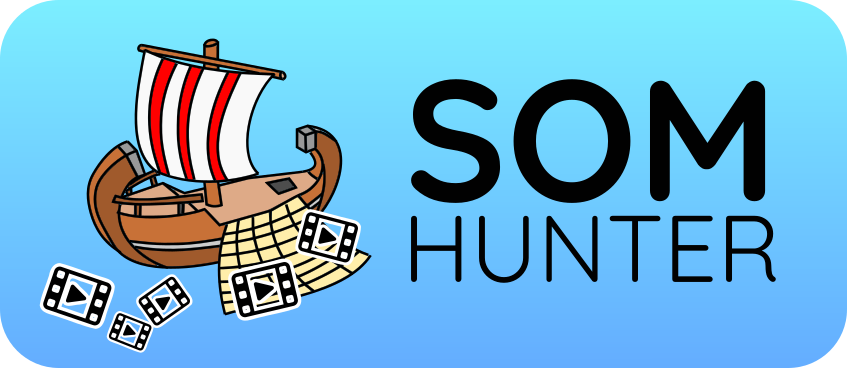
\includegraphics[width=0.7\textwidth]{img/somhunter-logo.png}
  \caption{\textbf{SOMHunter logo.}}
	\label{fig:logo}
\end{figure}


\section{SOMHunter Interface}
\label{sec:interface}

SOMHunter Tool has its user interface in the form web application. Thus you can use any modern browser to use it. Just visit the address where SOMHunter is running. In case you don't have that, ask your system administrator or visit developer documentation on how to build and launch the system.

After you open the beforementioned address, you should see the interface looking like \cref{fig:ui}.

\begin{figure}[h]
	\centering
	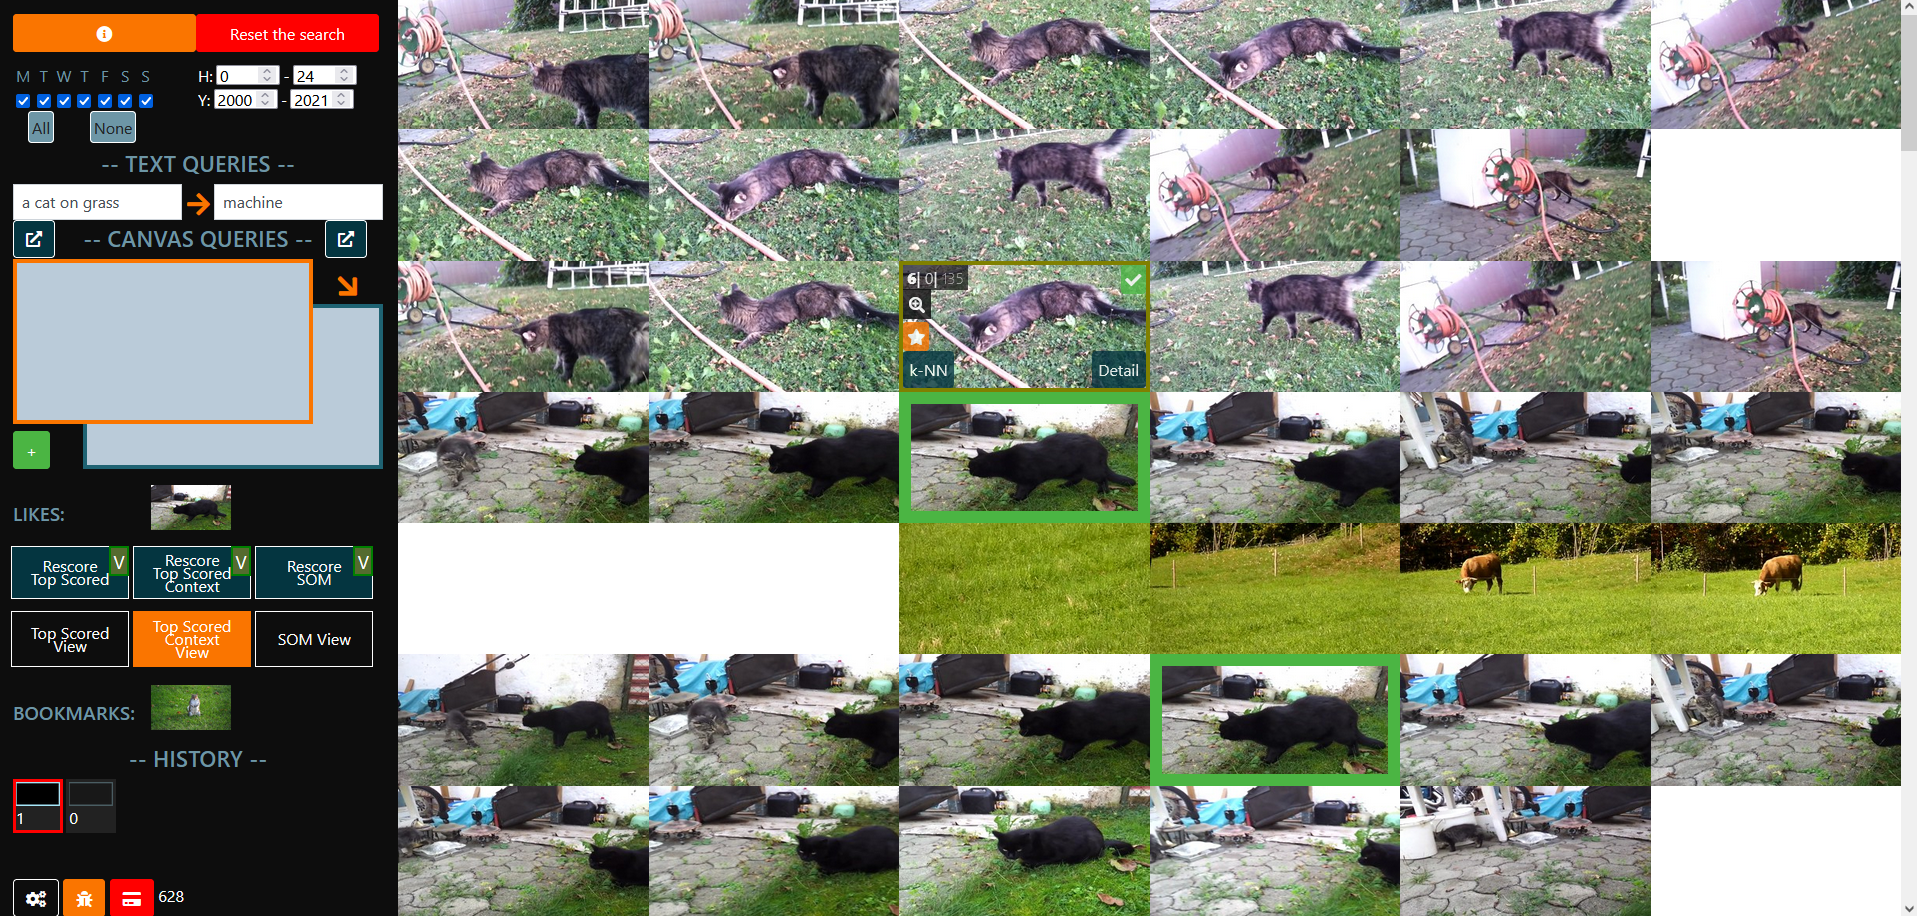
\includegraphics[width=1.0\textwidth]{img/ui.png}
  \caption{\textbf{SOMHunter Tool interface.}}
	\label{fig:ui}
\end{figure}


On the left side, there is the main panel, where you will construct the query and request rescores. The rest of the UI is current results displayed in a grid with the requested type of view (displays).  That is where you'll browse the results, provide the feedback by "liking" similar frames and look for the target scene(s).


%% %%%%%%%%%%%%%%%%%%%%%%%%%%%%%%%%%
\subsection{Textual Query}
\begin{figure}[h]
	\centering
	
\includegraphics[width=0.6\textwidth]{img/text-query.png}
  \caption{\textbf{Text querying interface panel.}}
	\label{fig:text-query}
\end{figure}

The textual querying is the most important part to formulate the query. There are two text inputs (see ~\cref{fig:text-query}) that allow you to formulate a so-called temporal query. That means that you are describing the two scenes that chronologically follow. For example, for the temporal query "A cat on a sofa" followed with "Dog barking at the door" we are describing part of the video with a scene where a cat is on a sofa followed with a scene of a barking dog.

As you can see, you can use natural language sentences to construct the queries. 


%% %%%%%%%%%%%%%%%%%%%%%%%%%%%%%%%%%
\subsection{Canvas Query}
\begin{figure}[h]
	\centering
  \begin{subfigure}[b]{0.45\textwidth}
      \centering
      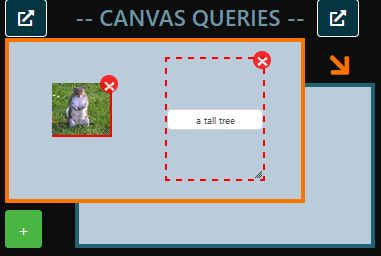
\includegraphics[width=\textwidth]{img/canvas-1.png}
      \caption{\textbf{Constructing the first canvas query.}}
  \end{subfigure}
  \hfill
  \begin{subfigure}[b]{0.45\textwidth}
      \centering
      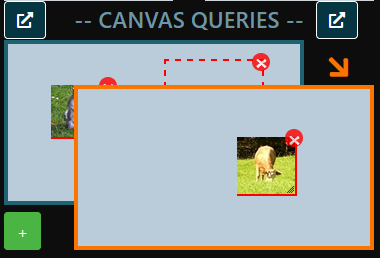
\includegraphics[width=\textwidth]{img/canvas-2.png}
      \caption{\textbf{Constructing the second canvas query.}}
  \end{subfigure}
	
  \caption{\textbf{Canvas querying interface panel}}
	\label{fig:canvas-query}
\end{figure}

The second option to formulate a temporal query is to use the canvases (see~\cref{fig:canvas-query}). With this, you have the advantage that you can specify approximate positions of the objects in the scene. Again the semantics of the temporality remains the same as in textual queries. Moreover, on a canvas, you can place both bitmaps and texts. 

To place a bitmap, just paste it from your clipboard by hitting Control+V (most GUIs of operating systems offer a keystroke to do create a rectangular snip from the screen directly to the clipboard; e.g. on Windows, it's Shift +Win + S). After that just reposition and scale it as you wish.

To place s text, hit the green plus button or do Shift + Left mouse click to the canvas. The textual input will appear. Just fill in the textual query, place and scale it as you require.


There are also some priorities in different query types for cases where (potentially) all the queries are used. The canvas query has a higher priority than the plain text query but is lower than query relocation. 

%% %%%%%%%%%%%%%%%%%%%%%%%%%%%%%%%%%
\subsection{Query Relocation}
\begin{figure}[h]
	\centering
	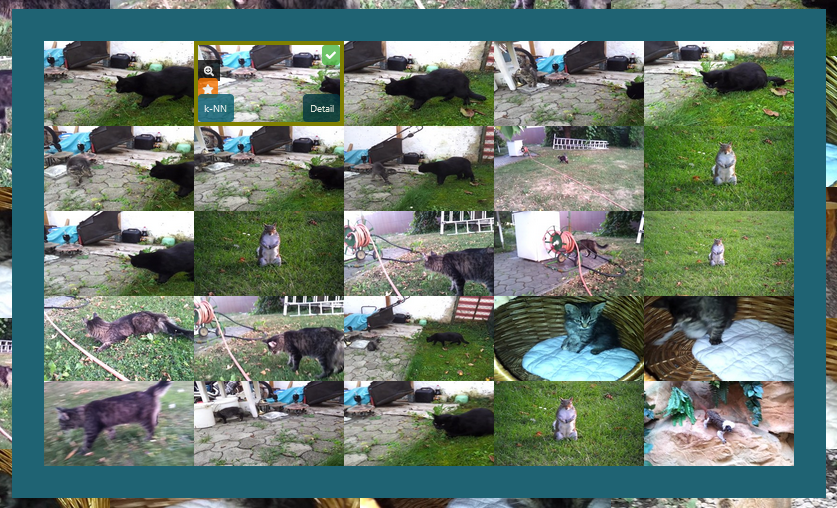
\includegraphics[width=0.5\textwidth]{img/relocation.png}
  \caption{\textbf{Relocation popup window.}}
	\label{fig:relocation}
\end{figure}

As an addition to other query-constructing methods, query relocation is primarily designed to make your current query more specific. Upon clicking on the arrow button under the textual inputs, you are prompted with a small grid of frames (see~\cref{fig:relocation}) where you can select the one that is the closest to what you are looking for.


To like a frame, just hover your mouse over it and click it with the left mouse button. Frames that are liked will have a green border around them and liked frames will also appear in liked panel (see figure).


%% %%%%%%%%%%%%%%%%%%%%%%%%%%%%%%%%%
\subsection{Likes}

SOMHunter has a relevance feedback model built in. That means that you can mark an arbitrary number of frames as "liked". After the next rescore, scores will be recomputed so they fit the feedback you have provided. This is an essential tool to solve difficult tasks. With this, you can iteratively get to the part of the database that you are interested in.

\begin{figure}[h]
	\centering
  \begin{subfigure}[b]{0.4\textwidth}
      \centering
      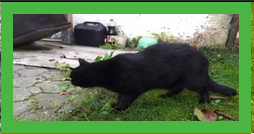
\includegraphics[width=\textwidth]{img/liked-frame.png}
      \caption{\textbf{Liked frames are marked as a wide green border.}}
      \label{fig:likes-a}
  \end{subfigure}
  \hfill
  \begin{subfigure}[b]{0.55\textwidth}
      \centering
      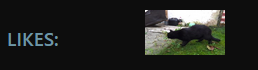
\includegraphics[width=\textwidth]{img/likes-panel.png}
      \caption{\textbf{Panel showing currently liked frames.}}
      \label{fig:likes-b}
  \end{subfigure}
	
  \caption{\textbf{Liking UI features.}}
	
\end{figure}

To like a frame, just hover your mouse over it and click it with the left mouse button. Frames that are liked will have a green border around them (see~\cref{fig:likes-a}) and liked frames will also appear in liked panel (see ~\cref{fig:likes-b}).

%% %%%%%%%%%%%%%%%%%%%%%%%%%%%%%%%%%
\subsection{Filters}
Filters are only available while working on certain datasets (e.g. Lifelog Search Challenge dataset). Such datasets contain also metadata based on what you can prune the frames that do not match the filters.

\begin{figure}[h]
	\centering
	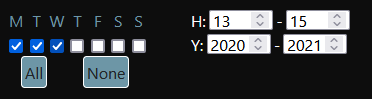
\includegraphics[width=0.6\textwidth]{img/filters.png}
  \caption{\textbf{Filtering UI panel.}}
	\label{fig:filters}
\end{figure}

As you can see on the figure, you can specify a year interval, hour interval and days in the week that the target scene belongs to. This is a hard filter therefore be careful with it so you don't filter out the scenes that may be the target. If frames are outside of the range of the filters they will never appear in the views (displays).


%% %%%%%%%%%%%%%%%%%%%%%%%%%%%%%%%%%
\subsection{Rescoring}
Whenever you are happy with your query, you have to ask the system to process it and give you the results based on your query. In case you used only the liking feature, the queries will accumulate and the previous state won't be reset. This is useful for iteratively getting closer to the target scene during difficult tasks.

To re-score, just hit one of the three buttons on rescore panel (see figure). All of them do the same rescore, they differ only in what display will be directly presented to you. 
The first one goes to a top-scored grid of frames. This is great for finding visually distinctive frames that are easy to spot.

\begin{figure}[h]
	\centering
	
\includegraphics[width=0.6\textwidth]{img/rescore-buttons.png}
  \caption{\textbf{Rescoring buttons.}}
	\label{fig:rescore}
\end{figure}

The second one goes to top-scored rows, where every row is just one result with the frame in the middle and its context before and after. This is a great view for catching scenes with some actions in them rather than just isolated frames.

The third one goes to the self-organized map display. This one is great for giving you a broader view of the database. For example when you're looking for some frames to like.

Each of the buttons has also the "V" button. That is because there are currently two textual models running in parallel. You can choose whether to use the default one (CLIP model) or the W2VV++ model. In some cases, they nicely complement each other so it may be helpful to try both of them. Please be aware that the CLIP model works only on plain text queries. The rest of the query types are handled by the W2VV++ model by default (likes as well).

After you re-score, the desired view is displayed to you. After that, you can switch between the views (displays) as you wish. While doing that you can keep your eyes peeled to spot some good frames to like.

%% %%%%%%%%%%%%%%%%%%%%%%%%%%%%%%%%%
\pagebreak
\subsection{Displays}

Displays are different views of the current distribution of scores. In other words, switching displays does not modify the query or scores in any way. 
There are multiple displays to offer you a variety of different approaches.
The general grid views are accessible through the panel (see~\cref{fig:display-buttons}) and the rest of them are on the frame overlay (see~\cref{fig:frame-overlay}). The numbers in the top left corner of the overlay indicate video ID, shot ID and frame number respectively.

\begin{figure}[h]
	\centering
  \begin{subfigure}[b]{0.6\textwidth}
      \centering
      
\includegraphics[width=\textwidth]{img/view-buttons.png}
      \caption{\textbf{Buttons to switch to the three main displays.}}
      \label{fig:display-buttons}
  \end{subfigure}
  \hfill
  \begin{subfigure}[b]{0.35\textwidth}
      \centering
      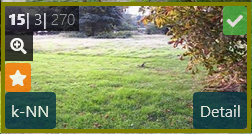
\includegraphics[width=\textwidth]{img/frame-overlay.png}
      \caption{\textbf{Frame overlay showed on mouse hover.}}
      \label{fig:frame-overlay}
  \end{subfigure}
	
  \caption{\textbf{UI elements related to changing views.}}
	
\end{figure}

Always remember that the Esc key closes any popups that may apear. That is the fastest way to close them.

\pagebreak
\subsubsection{Top-scored Display}
This display (see~\cref{fig:top-display}) just shows you a grid of frames that currently have the highest scores. Ordered from the one with the highest score to the lowest. Use this display to look for visually distinct frames that are easy to spot.

\begin{figure}[h]
	\centering
	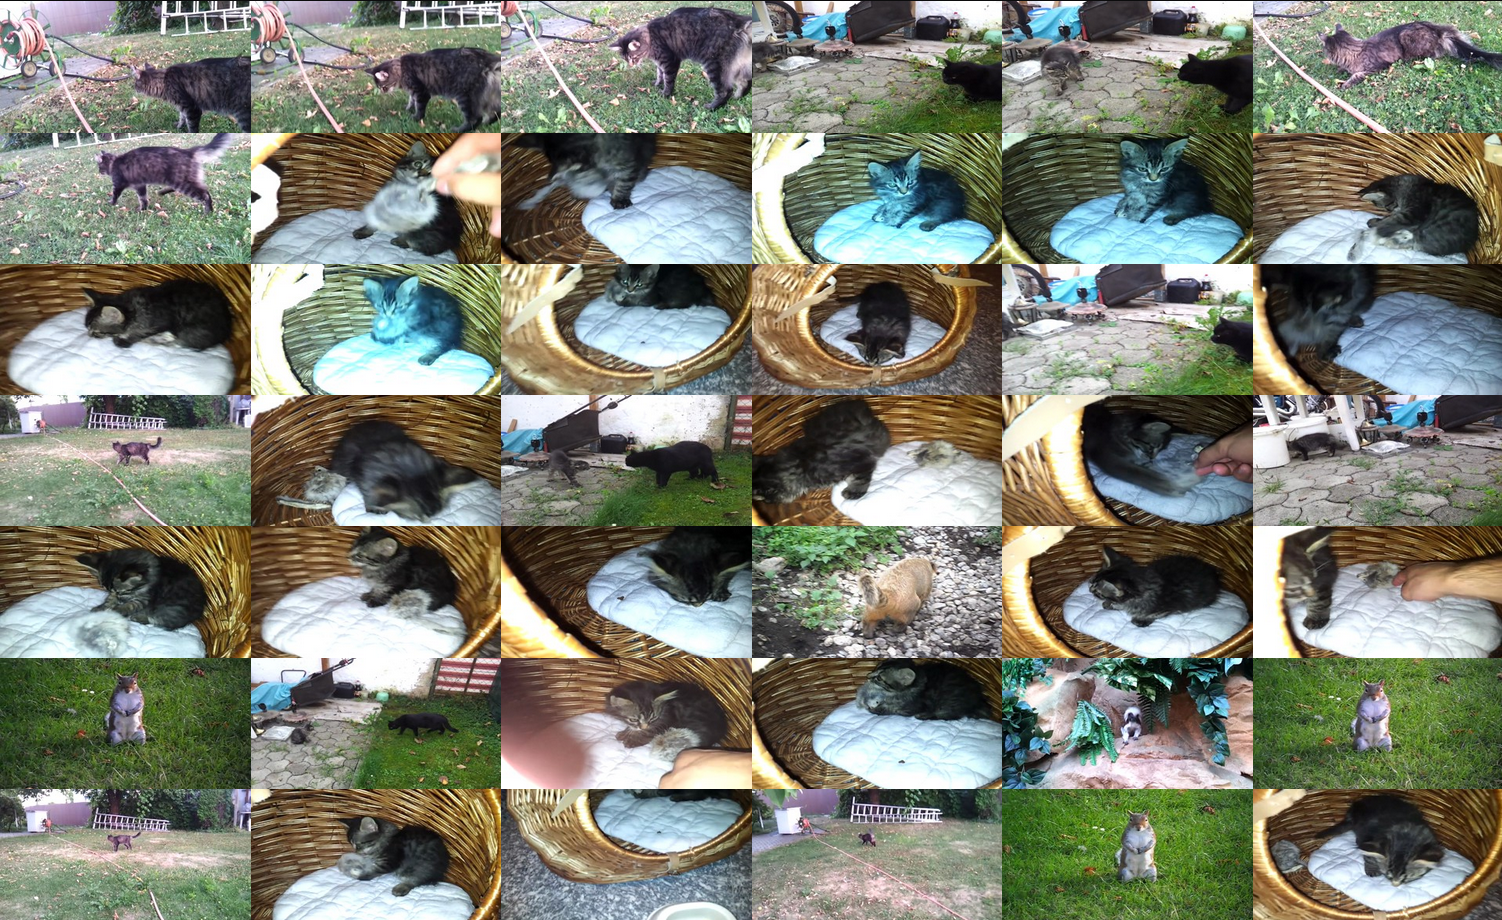
\includegraphics[width=1.0\textwidth]{img/top.png}
  \caption{\textbf{An example of top-scored display.}}
	\label{fig:top-display}
\end{figure}

\pagebreak
\subsubsection{Top-scored Context Display}
This display is the extension of the top-scored display. It basically shows the same top-scored frames, but puts them into the context (see~\cref{fig:top--context-display}). That means that each row is just one result where the frame itself is in the middle column and you can see the frames that preceded and those which succeeded. This is a great tool to browse for shots with some chronological progress.

\begin{figure}[h]
	\centering
	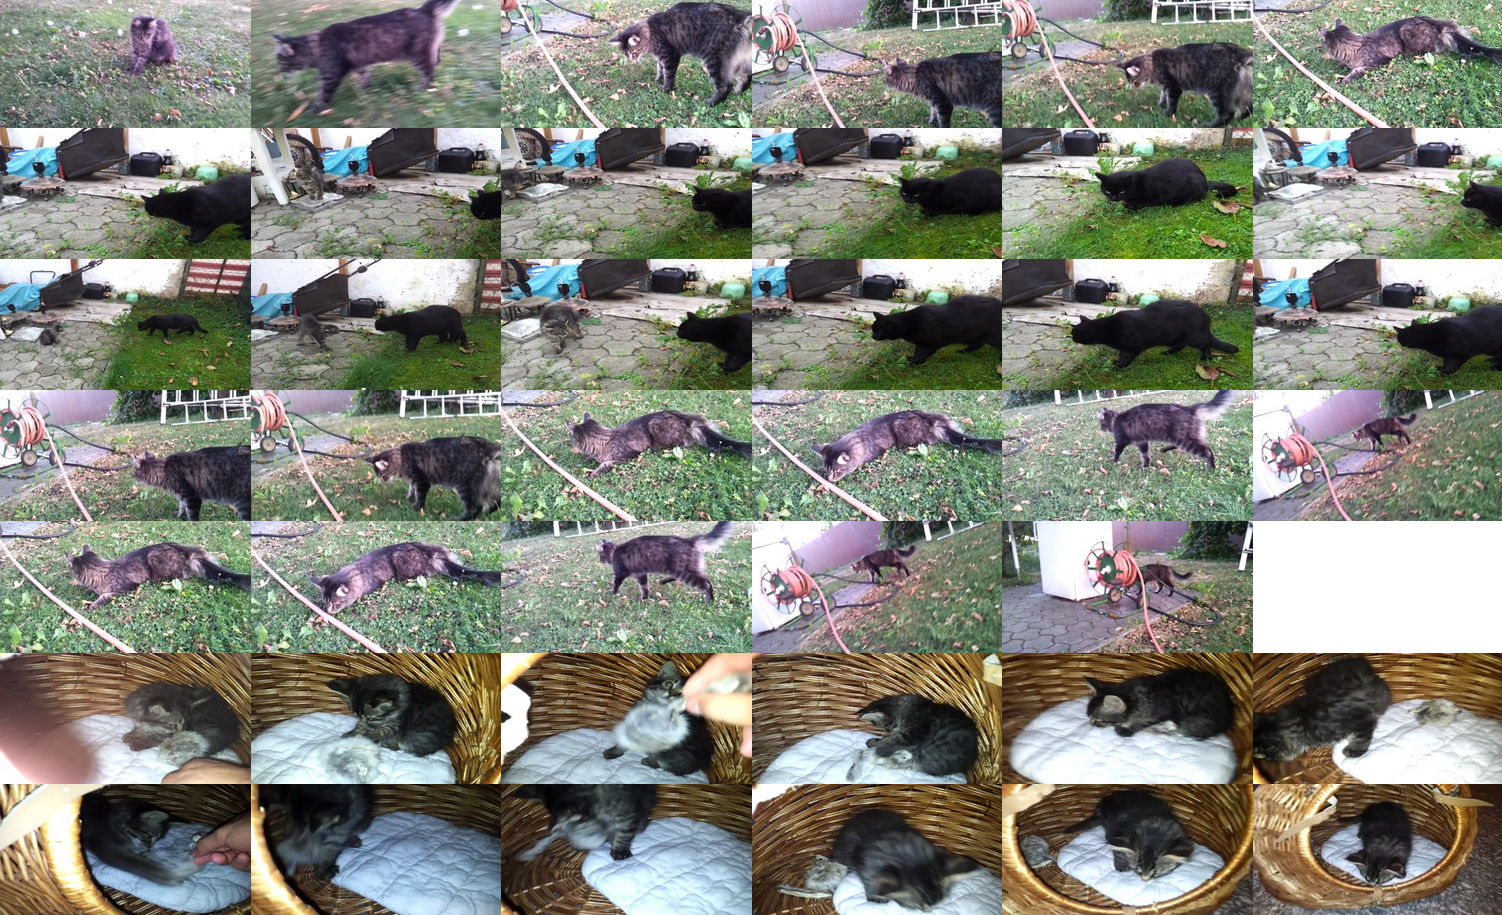
\includegraphics[width=1.0\textwidth]{img/top-context.png}
  \caption{\textbf{An example of a top-scored context display.}}
	\label{fig:top--context-display}
\end{figure}

\pagebreak
\subsubsection{SOM Display}
This display is based on self-organizing map and thus clusters together similar frames (see~\cref{fig:som-display}). It is a great tool to give you a broader view to the distribution of current dataset scores. You can switch here to find good example frames to like and provide valuable feedback to the model.

\begin{figure}[h]
	\centering
	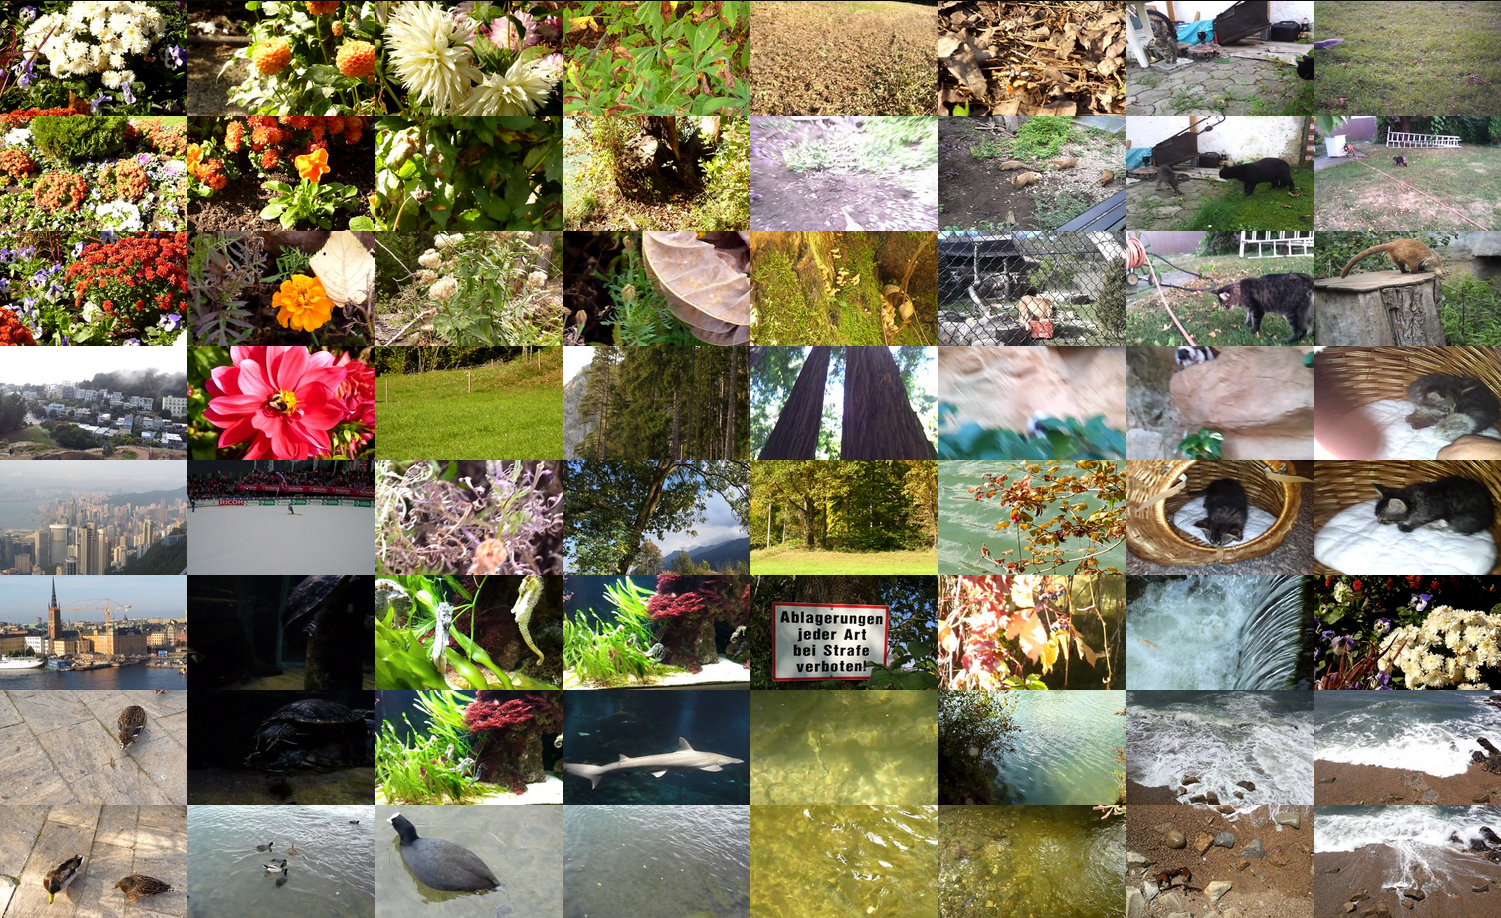
\includegraphics[width=1.0\textwidth]{img/som-display.png}
  \caption{\textbf{An example of a SOM display.}}
	\label{fig:som-display}
\end{figure}

\subsubsection{Nearest Neighbours Display}
You can show nearest neighbour frames for each of the frames in the dataset. This display shows exactly what it says. No catches here. To show nearest neighbours just click the "k-NN" button on the frame overlay (see~\cref{fig:frame-overlay}).

\pagebreak
\subsubsection{Video Detail}
Often you need to inspect the whole video to see if it's the one you're looking for. Just click the "Detail" button on the frame overlay and the video detail window will show up. It shows all dataset frames from the given video. The frame with a red border is the one you jumped to this window through.

Once you inspected some video like this, all the frames from this video will get a slight fadeout so you can clearly see what frames are of smaller importance since you already inspected them. This effect is reset when the search is reset (see~\cref{par:reset}).

\begin{figure}[h]
	\centering
	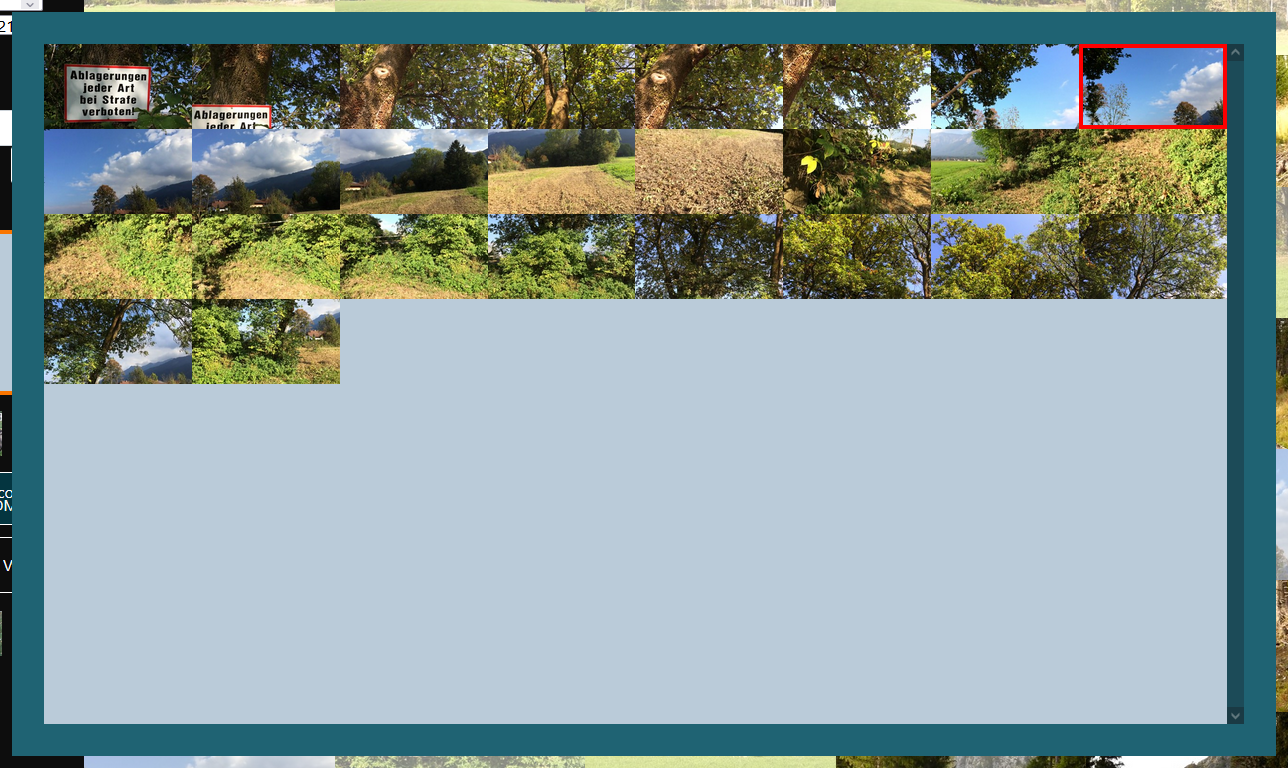
\includegraphics[width=1.0\textwidth]{img/detail-window.png}
  \caption{\textbf{An example of a detail window.}}
	\label{fig:detail-window}
\end{figure}

\subsubsection{Video Replay}
Whenever you need to just see the wider context to the frame you are seeing, you can Shift + Mouse Wheel on top of that screen to scroll through its frames (see~\cref{fig:replay-overlay}). The frame with a red border is the one you started the replay through.

\begin{figure}[h]
	\centering
	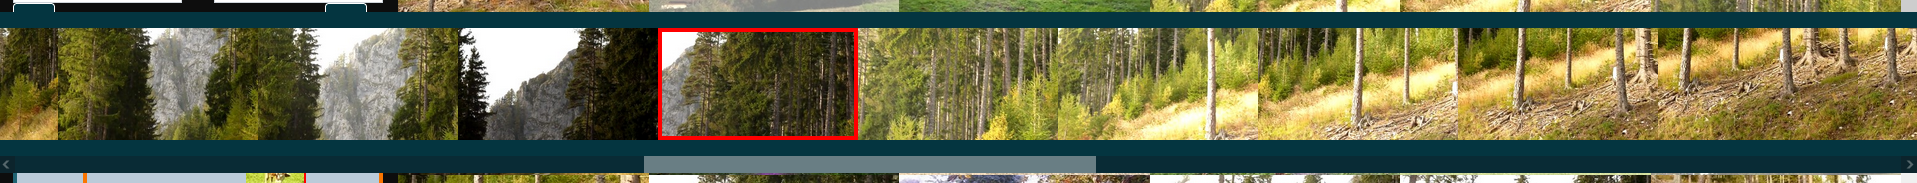
\includegraphics[width=1.0\textwidth]{img/replay-overlay.png}
  \caption{\textbf{An example of a replay slider.}}
	\label{fig:replay-overlay}
\end{figure}

\subsubsection{Zoom Display}
Sometimes we need to see some details in the frame. Just click the magnifying glass icon on its overlay or Shift + Left click it. This will show the zoomed version of the frame (see~\cref{fig:zoom}).

\begin{figure}[h]
	\centering
	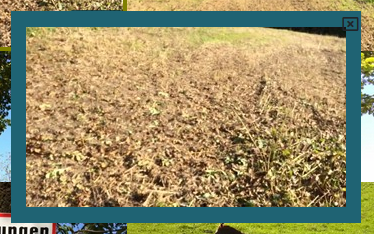
\includegraphics[width=0.5\textwidth]{img/zoom.png}
  \caption{\textbf{An example of a zoomed frame.}}
	\label{fig:zoom}
\end{figure}

%% %%%%%%%%%%%%%%%%%%%%%%%%%%%%%%%%%
\subsection{History}
From time to time it may come handy to "go back in time" (for example you reformulate your query in a way that the previous one was better). At any time, you can jump back to any search state you were in. That means that every re-score creates checkpoint of that state in that time. Whenever you switch to any history point, you can change displays as you wish. You can even add relevance feedback to that state and continue from it. The new point will be added to the top of the stack. The checkpoints are accessible from the history panel (see~\cref{fig:history}) by just clicking on them.

History is reset with the search reset.

\begin{figure}[h]
	\centering
	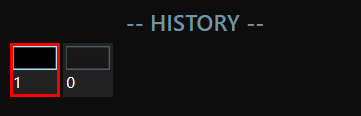
\includegraphics[width=0.6\textwidth]{img/history-panel.png}
  \caption{\textbf{History panel.}}
	\label{fig:history}
\end{figure}

%% %%%%%%%%%%%%%%%%%%%%%%%%%%%%%%%%%
\subsection{Bookmarks}
Bookmarks serve as a way how to store frames that you might need in the future. An example of such a situation is when you're not sure that what you found is the correct one. You can bookmark a frame by clicking a star icon on a frame overlay (see~\cref{fig:bookmarks}). 

Bookmarks are reset with the reset, just as history is.

\begin{figure}[h]
	\centering
	
\includegraphics[width=0.6\textwidth]{img/bookmarks-panel.png}
  \caption{\textbf{Bookmarks panel.}}
	\label{fig:bookmarks}
\end{figure}

%% %%%%%%%%%%%%%%%%%%%%%%%%%%%%%%%%%
\subsection{Other Utilites}
\paragraph{Reset Search}
\label{par:reset}
To reset the search, just click the "Reset the search" button in the top left part of the screen.

\paragraph{Submit to the Competition Server}
During the competition participation (e.g. LSC, VBS) you need to submit the correct segment to the competition server. Our system currently supports the DRES server and an older version VBS Server (DRES by default). 

To submit, just click the green "check" button in the top right corner of the frame overlay. You will get a small notification in the top right corner.

\paragraph{Log in to the Competition Server}
The system logs in to the competition server during the launch. But sometimes when there is a restart of the competition server, you need to log in again to the server. Just click the "cogwheel" button at the bottom of the left panel and hit "Login to the server". After that, you should get a confirming prompt. 






\section{Usage}
\label{sec:usage}




% \bibliography{biblio} 
% \bibliographystyle{apalike}

% \printindex
% \begin{appendices}

% \end{appendices}


\end{document}
